\documentclass[review]{elsarticle}

\usepackage{lineno,hyperref}
\modulolinenumbers[5]

% for alg.
\usepackage{algorithm}
\usepackage{algpseudocode}
\usepackage{enumitem}
\usepackage{balance}
\def\algbackskip{\hskip\dimexpr-\algorithmicindent+\labelsep}
\def\LState{\State \algbackskip}

% for table.
\usepackage{multirow, array, amsmath}

\journal{Journal of \LaTeX\ Templates}

%%%%%%%%%%%%%%%%%%%%%%%
%% Elsevier bibliography styles
%%%%%%%%%%%%%%%%%%%%%%%
%% To change the style, put a % in front of the second line of the current style and
%% remove the % from the second line of the style you would like to use.
%%%%%%%%%%%%%%%%%%%%%%%

%% Numbered
%\bibliographystyle{model1-num-names}

%% Numbered without titles
%\bibliographystyle{model1a-num-names}

%% Harvard
%\bibliographystyle{model2-names.bst}\biboptions{authoryear}

%% Vancouver numbered
%\usepackage{numcompress}\bibliographystyle{model3-num-names}

%% Vancouver name/year
%\usepackage{numcompress}\bibliographystyle{model4-names}\biboptions{authoryear}

%% APA style
%\bibliographystyle{model5-names}\biboptions{authoryear}

%% AMA style
%\usepackage{numcompress}\bibliographystyle{model6-num-names}

%% `Elsevier LaTeX' style
\bibliographystyle{elsarticle-num}
%%%%%%%%%%%%%%%%%%%%%%%

\begin{document}

\begin{frontmatter}

\title{IGCF: Instance Guided Correlation Filter}
\tnotetext[mytitlenote]{Fully documented templates are available in the elsarticle package on \href{http://www.ctan.org/tex-archive/macros/latex/contrib/elsarticle}{CTAN}.}

%% Group authors per affiliation:
\author{Zhenbang Li\fnref{myfootnote}, Qiang Wang, Jin Gao, Bing Li, Weiming Hu}
\address{Radarweg 29, Amsterdam}
\fntext[myfootnote]{Since 1880.}

%% or include affiliations in footnotes:
\author[mymainaddress,mysecondaryaddress]{Elsevier Inc}
\ead[url]{www.elsevier.com}

\author[mysecondaryaddress]{Global Customer Service\corref{mycorrespondingauthor}}
\cortext[mycorrespondingauthor]{Corresponding author}
\ead{support@elsevier.com}

\address[mymainaddress]{1600 John F Kennedy Boulevard, Philadelphia}
\address[mysecondaryaddress]{360 Park Avenue South, New York}

\begin{abstract}
Traditional correlation filter (CF) based trackers typically rely only on ridge regression for online learning without the perception of instance level information of objects, which may lead to drift and failure of CF trackers. In this paper, we propose the Instance Guided Correlation Filter (IGCF) to improve the tracking robustness. Specifically, a deep network called InstMask is designed to generate the instance mask of objects, which are used to explicitly constraint the learning process of correlation filters. Based on the instance-level segmentation, we further propose a self-correction mechanism to mitigate the drift problem of CF trackers. Extensive experiments on several challenging benchmarks demonstrate that our IGCF tracker performs favorably against state-of-the-art trackers while running on a single CPU core at 5 FPS.
\end{abstract}

\begin{keyword}
CNN \sep object tracking \sep DCF \sep self-correction
\MSC[2010] 00-01\sep  99-00
\end{keyword}

\end{frontmatter}

\linenumbers

\section{Introduction}
Object tracking is a fundamental topic in computer vision. Given the initialized state of an object in the starting frame of a video, the aim of tracking is to estimate the states of the object in the subsequent frames. Extensive studies \cite{Bolme2010VisualOT, Danelljan2014AccurateSE, Henriques2015HighSpeedTW, Li2014ASA, Nam2016LearningMC, Danelljan2015ConvolutionalFF, Wang2018SiamMask} have been carried out to address the challenges in object tracking, such as occlusion, illumination change, appearance change, fast motion and so on. Recently, there has been a surge of interest in discriminative correlation filter (DCF) approaches \cite{Bolme2010VisualOT, Danelljan2014AccurateSE, Henriques2015HighSpeedTW, Li2014ASA} which can efficiently utilize all spatial shifts of the training samples by exploiting the discrete Fourier transform. However, most of DCF trackers can not perceive the instance level information of objects, which causes the the object to be represented only by a rough rectangular box. For irregularly shaped objects or those with a hollow center, the rectangular object regions will be doped with more background information, which may lead the tracker to drift and failure. Besides, the DCF trackers are often restricted to low-level features, significantly limiting its potential. Several CNN-based trackers \cite{Nam2016LearningMC, Danelljan2015ConvolutionalFF} have demonstrated the performance advantages of deep learning. However, these trackers also face the problem of lack of instance level information. Due to the inability of integrating target-specific information, most CNN based trackers do not provide a powerful model update strategy, resulting in inferior robustness. Furthermore, CNN-based trackers are often computationally expensive, making it difficult to run efficiently on the CPU. 

\begin{figure} 
    \subfig{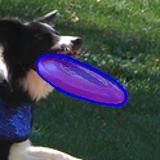
\includegraphics[width=2.4cm]{images/coco/00893.jpg}}          \hspace{-0.6em}        
    \subfig{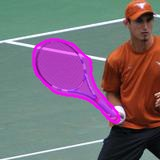
\includegraphics[width=2.4cm]{images/coco/01107.jpg}}          \hspace{-0.6em}        
    \subfig{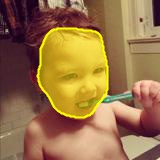
\includegraphics[width=2.4cm]{images/coco/01108.jpg}}          \hspace{-0.6em}        
    \subfig{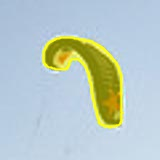
\includegraphics[width=2.4cm]{images/coco/01564.jpg}}          \hspace{-0.6em}        
    \subfig{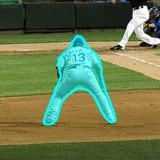
\includegraphics[width=2.4cm]{images/coco/01664.jpg}}\\[0.2ex]
    \subfig{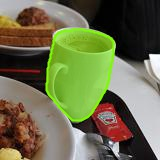
\includegraphics[width=2.4cm]{images/coco/01939.jpg}}                     \hspace{-0.6em}
    \subfig{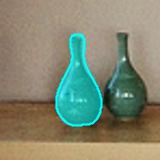
\includegraphics[width=2.4cm]{images/coco/02078.jpg}}                     \hspace{-0.6em}
    \subfig{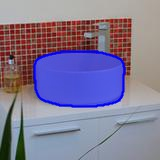
\includegraphics[width=2.4cm]{images/coco/02285.jpg}}                     \hspace{-0.6em}
    \subfig{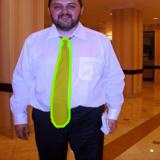
\includegraphics[width=2.4cm]{images/coco/02497.jpg}}                     \hspace{-0.6em}
    \subfig{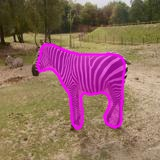
\includegraphics[width=2.4cm]{images/coco/02589.jpg}}\\[0.2ex]
    \subfig{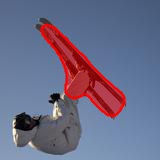
\includegraphics[width=2.4cm]{images/coco/02700.jpg}}                   \hspace{-0.6em}
    \subfig{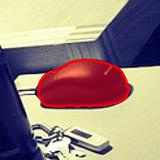
\includegraphics[width=2.4cm]{images/coco/03000.jpg}}                   \hspace{-0.6em}
    \subfig{
\includegraphics[width=2.4cm]{images/coco/03327.jpg}}                   \hspace{-0.6em}
    \subfig{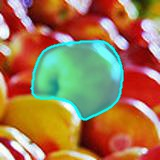
\includegraphics[width=2.4cm]{images/coco/03482.jpg}}                   \hspace{-0.6em}
    \subfig{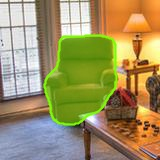
\includegraphics[width=2.4cm]{images/coco/03733.jpg}}
    \caption{Segmentation results of InstMask on COCO2017 \cite{Lin2014MicrosoftCC} val dataset.}
    \label{fig:InstMask}
\end{figure}

In this work, we propose the Instance Guided Correlation Filter (IGCF), that directly addresses all aforementioned limitations. Specifically, a deep network called InstMask is designed to generate the instance mask of objects, which are used to explicitly constraint the learning process of correlation filters. The instance mask can suppress the interference of background information in the positive samples during training. In order to obtain accurate and semantic segmentation results (see Fig. \ref{fig:InstMask}), we use the data-driven approach to generate instance-level masks. Unlike common object segmentation tasks, we have designed new network structures and training methods that enable InstMask to identify salient objects of any category located in the center of the image patch, instead of identifying image categories only in the training set. Besides, we discover that the DCF result updated online and the InstMask result with high-level semantic attributes are independent and complementary, so they can be integrated together to further improve tracking accuracy. Specifically, based on the instance-level segmentation, we further propose a self-correction mechanism to mitigate the drift problem of CF trackers. The geometric center of the segmentation mask is used to correct the prediction bias of the correlation filter. Equipped with the InstMask module, the proposed IGCF not only performs the object tracking task well, but also can be used for the task of video object segmentation, which demonstrates the wide application space of this algorithm. The architecture of the proposed tracking framework IGCF is shown in Fig. \ref{fig:IGCF}.

\begin{figure*}
    \centering
    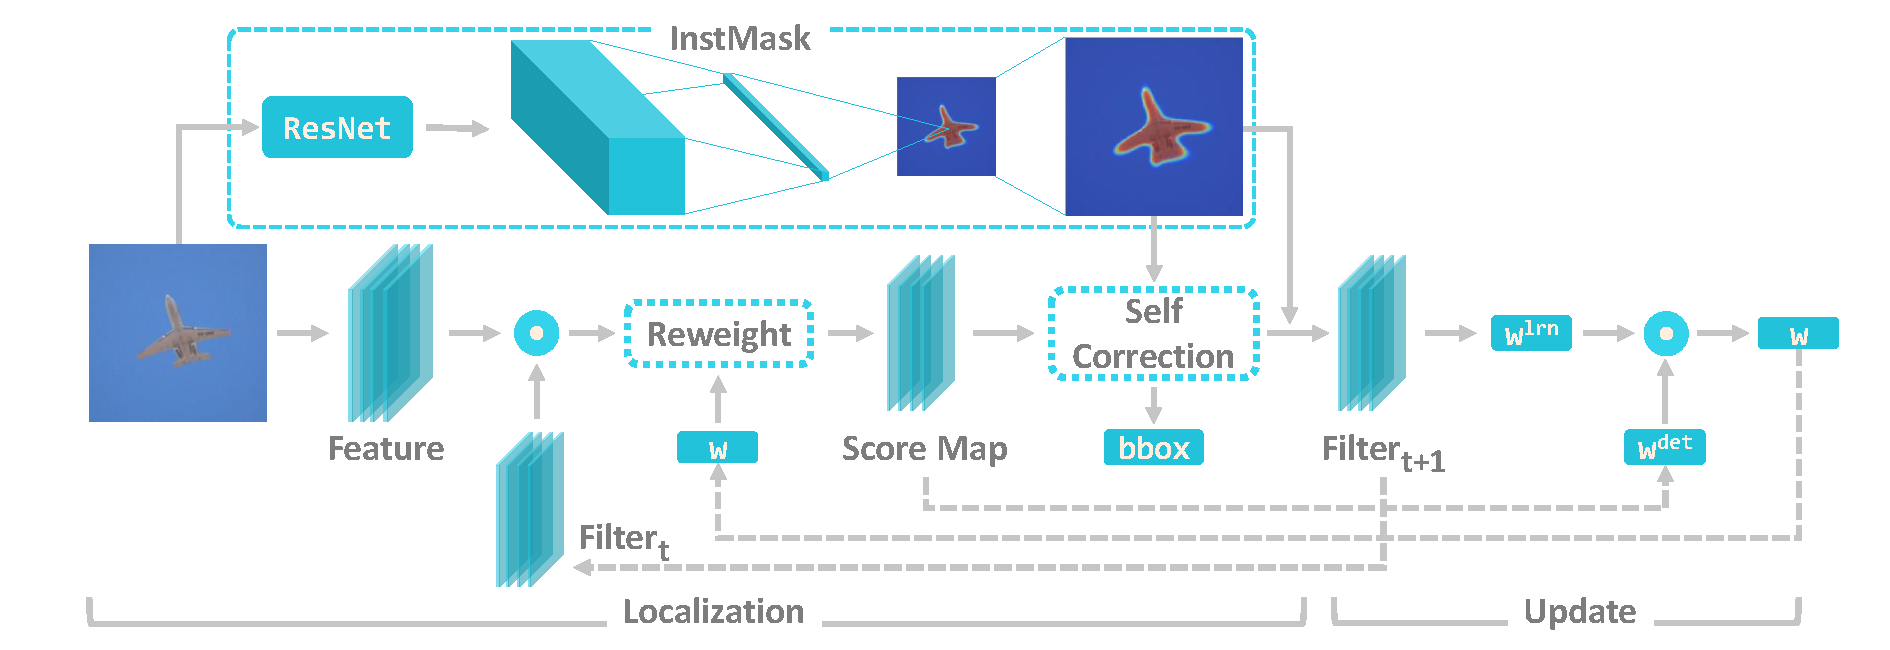
\includegraphics[width=12cm]{images/instmask.pdf}
    \caption{Architecture of the tracking framework IGCF.}
    \label{fig:IGCF}
\end{figure*}

We perform comprehensive experiments on three tracking benchmarks: VOT2015 \cite{Kristan2015TheVO}, VOT2016 \cite{Kristan2016TheVO} and GOT-10K \cite{Huang2018GOT10kAL}. Our IGCF tracker performs favorably against state-of-the-art trackers while running on a single CPU core at 5 FPS. Finally, we perform qualitative experiments on the video object segmentation dataset DAVIS2016 \cite{Perazzi2016}, showing the powerful semantic segmentation and tracking capabilities of our algorithm.

\section{Related works}
The development of object tracking has a history of decades. Generally speaking, the goal of object tracking is to establish the positional relationship of the object to be tracked in a continuous video sequence, and obtain the complete motion trajectory of the object. In other words, given the target coordinate position of the first frame of the image, the exact positions of the target in the subsequent frames are calculated by the tracker. 

\subsection{Traditional trackers}
Many traditional object tracking algorithms are designed to solve the challenges in object tracking, such as partial occlusion, illumination variation, background clutter, motion blur, viewpoint change as so on.
In TLD \cite{kalal2011tracking}, the long-term tracking problem is decomposed into three subtasks: tracking, learning and detection. The tracker follows the object from frame to frame. The detector localizes all appearances that have been observed so far and corrects the tracker if necessary. The learning estimates detector’ s errors and updates it to avoid these errors in the future. 
\cite{Bolme2010VisualOT} proposed a traker based on Minimum Output Sum of Squared Error (MOSSE) filters, which is robust to variations in lighting, scale, pose, and non-rigid deformations while operating at 669 frames per second.
CSK \cite{Henriques2012ExploitingTC} improves the MOSSE filter by adopting the circulant structure of subwindows of an image, which use the Fast Fourier Transform (FFT) to quickly incorporate information from all subwindows. Additionally, CSK also shows that classification on non-linear feature spaces with the Kernel Trick can be done as efficiently as in the original image space. However, the CSK tracker using only grayscale samples to train the filter.
Based on SCK, \cite{Danelljan2014AdaptiveCA} has shown a notable improvement by learning multi-channel filters on multi-dimensional color attributes. To avoid the extra computational overhead caused by the high dimensionality of color attributes, \cite{Danelljan2014AdaptiveCA} proposed an adaptive dimensionality reduction technique which reduces the original eleven dimensions to only two.
KCF \cite{Henriques2015HighSpeedTW} proposed an analytic model for datasets of thousands of translated patches, which can be diagonalized with the Discrete Fourier Transform. This operation can reduce both storage and computation by several orders of magnitude.
To avoid the boundary effects caused by the periodic assumption of the training and detection samples in the standard DCF formulation, \cite{Danelljan2015LearningSR} proposed Spatially Regularized Discriminative Correlation Filters (SRDCF), which introduced a spatial regularization component in the learning to penalize correlation filter coefficients depending on their spatial location.
CSR-DCF \cite{Lukezic2017DiscriminativeCF} introduces the channel and spatial reliability components to DCF tracking and provides a learning algorithm for its efficient and seamless integration in the filter update and the tracking process. The spatial reliability component adjusts the filter support to the part of the object suitable for tracking. The channel reliability component reflects channel-wise quality of the learned filters and is used as feature weighting coefficients in localization.
Struck \cite{Hare2011StruckSO} presented a framework for adaptive visual object tracking based on structured output prediction. It avoids the need for an intermediate classification step by explicitly allowing the output space to express the needs of the tracker.
Despite the attractive performance both in accuracy and robustness, most correlation filter-based trackers use the template with the fixed size, which is not able to handle the scale changes of a target. In order to solve the scale change problem, \cite{Li2014ASA} sample the target with different scales, and adjust the samples into a fixed size for comparison with the leant model at each frame. Meanwhile, \cite{Li2014ASA} adopt a multiple feature integration scheme, which employs the raw pixel, Histogram of Gradient \cite{Forsyth2014ObjectDW} and color-naming \cite{Weijer2009LearningCN} to further enhance the tracker.
\cite{Danelljan2017DiscriminativeSS} learns discriminative correlation filterse based on a pyramid representation to perform scale estimation. The 1-dimensinal filters are used for estimating the scale only, 2-dimensional filters for translation only and 3-dimitional filters for exhaustive scale-space localization of the target.
Staple (Sum of Template And  Pixel-wise LEarners) \cite{Bertinetto2016StapleC} combines complementary cues to improve the robustness of the tracker, which not only utilizes the template model to deal with motion blur and illumination changes, but also uses color distributions to cope with deformation. To maintain real-time speed, Staple solve two independent ridge-regression problems, exploiting the inherent structure of each representation.

\subsection{CNN based trackers}
In the past few years, deep learning \cite{Goodfellow2015DeepL} has achieved remarkable success in many research fields, especially in computer vision \cite{Girshick2016RegionBasedCN, Schroff2015FaceNetAU}, speech recognition \cite{Kim2016JointCB, Wu2015DeepNN} and natural language processing \cite{Vinyals2014GrammarAA, Bahdanau2014NeuralMT}. Several deep-learning-based trackers have demonstrated the performance advantages of deep learning. 
Most DCF-based trakers is restricted to single-resolution feature maps, significantly limiting its potential. To solve this problem, CCOT \cite{Danelljan2016BeyondCF} learns continuous convolution filters to fuse the feature maps with different resolution, which produces the continuous-domain confidence map for the target. In addition to multi-resolution fusion, the continuous domain learning formulation enables accurate sub-pixel localization.
GoTurn \cite{held2016learning} proposed a method for offline training of neural networks that can track objects at test-time at 100 fps. It uses a simple feed-forward network with no online training required, which learns a generic relationship between object motion and appearance and can be used to track novel objects that do not appear in the training set. 
Recently, a series of work such as SiamFC \cite{bertinetto2016fully}, SiamRPN \cite{Li2018HighPV} and DasiamRPN \cite{zhu2018distractor}, use the siamese network to learn the similarity of search images and exemplar images, which can achieve a good balance between speed and accuracy. 
SANet \cite{Fan2016SANetSN} uses selfstructure information of the object to distinguish it from distractors. Specifically, It utilizes recurrent neural network (RNN) to model object structure, and incorporate it into CNN to improve its robustness to similar distractors. 
In \cite{fan2017parallel}, the tracking framework consists of two components, a tracker and a verifier, working in parallel on two separate threads. The tracker aims to provide a super real-time tracking inference and is expected to perform well most of the time; by contrast, the verifierchecks the tracking results and corrects the tracker when needed. 
In \cite{supancic2017tracking}, the author proposes to learn an optimal decision-making policy by formulating tracking as a partially observable decisionmaking process. 
In \cite{yun2017action}, the author proposes a tracker to pursue the change of target by repetitive actions controlled by the proposed action-decision network, which can achieve a light computation as well as satisfactory tracking accuracy in both location and scale.

\section{The Proposed Method}

\subsection{InstMask} \label{sec:InstMask}
DCF trackers \cite{Bolme2010VisualOT, Danelljan2014AccurateSE, Henriques2015HighSpeedTW, Li2014ASA} have been widely studied and used in object tracking area. Specifically, consider the appearance feature: $f=\{f_d\}_{d=1:N_c}$ of an object, where $N_c$ is the channel number of the object feature. The goal of DCF-like trackers is to train a filter $h=\{h_d\}_{d=1:N_c}$, such that the correlation response between the feature and the filter can fit the desired output $g$ which is typically a 2-D Gaussian function centered at the target location: 
\begin{equation} \label{eq:dcf}
\tilde{g}=\sum_{d=1}^{N_c}f_d \star h_d \cdot w_d,
\end{equation}
where $\star$ represents the circular correlation operator and channel weights $w = \{w_d\}_{d=1:N_c}$ are the scaling factors based on the discriminative power of each feature channel \cite{Lukezic2017DiscriminativeCF}.
The position of the peak of the response map is regarded as the object position in the current frame.
The optimal correlation filter $h$ is estimated by minimizing:
\begin{equation}
\varepsilon(h) = \sum_{d=1}^{N_c}||f_d \star h_d - g||^2+\lambda||h_d||^2.
\end{equation}

As described in CSRDCF \cite{Lukezic2017DiscriminativeCF}, segmentation masks can be utilized to improve tracking performance. The segmentation mask of an image patch is a spatial map with elements either 1 or 0, that indicates whether pixels belong to the object in the image patch or belong to the background. During the filter training process, the filter $h$ is constrained by the mask $m$: $h \equiv m \odot h$. This constraint adapts the filter support to the part of object suitable for tracking, which enables a large training region to capture more context information and overcomes the limitations related to the rectangular shape assumption.

In CSRDCF \cite{Lukezic2017DiscriminativeCF}, the segmentation masks are generated using the color histograms of the object foreground and background. This heuristic approach has several disadvantages: (1) Since only low-level pixel information is used, it is difficult to accurately segment an object. (2) The CSRDCF uses unreliable positional prior information to adjust the inaccurate segmentation results, which introduces further errors in some complex tracking scenarios. (3) In order to adapt to the apparent changes of the object, the histogram model is constantly updated during the tracking process, which easily leads to drift of the tracker.

For the sake of solving the above problems, we propose a concise way to generate object segmentation masks instead of iterative optimization for color histogram. Compared with CSRDCF, our approach need not  online update the color histogram, which improves computational efficiency while avoiding the undesired drift. Besides, tracking results are more accurate because of the use of semantic level rather than pixel-level information for segmentation.

\textbf{Architecture} We propose to learn a fully convolutional network that returns the segmentation mask for the saliency object in a certain frame. To meet the needs of object tracking, there are several differences between InstMask and traditional object segmentation network. First, the InstMask is designed as a saliency object detector to capture the object mask in the search region. Consequently InstMask works as a class-agnostic segmentation network. Although InstMask uses COCO dataset \cite{Lin2014MicrosoftCC} with only 80 classes for training, the network is able to segment categories that do not appear in the training set, as shown in Fig. \ref{fig:IGSC}. Second, during tracking, the object position is assumed to be in the vicinity of the object position in the previous frame. So the input to InstMask is always the image region centered on the object position at the previous frame.

The network architecture is shown in Table \ref{tab:InstMask}. The backbone of InstMask is constructed based on ResNet50 \cite{He2016DeepRL}, which consists of a stem block and 3 residual blocks.
The input of InstMask is a 160$\times$160$\times$3 image patch. It is sent to the stem block, producing a 80$\times$80$\times$64 feature map. Then the feature map is sent to 3 residual blocks sequentially, producing feature maps of size 40$\times$40$\times$256, 20$\times$20$\times$512, 10$\times$10$\times$1024, respectively. Subsequently, the obtained feature map is sent to 3 convolution layers to generate the segmentation mask vector of length 3136. Finally, this vector is reshaped to 56$\times$56 to get the final segmentation mask.

\begin{algorithm}
  \caption{The IGCF tracking algorithm.} 
  \begin{algorithmic}
    \Require Image $I_t$, object position on previous frame $p_{t-1}$, scale $s_{t-1}$, filter $h_{t-1}$, channel reliability $w_{t-1}$.
    \Ensure Position $p_t$, scale $s_t$ and updated models.
  \Statex
  \LState \textbf{Localization:}
  \begin{enumerate}[leftmargin=0pt,itemindent=1.5em]
    \item $p_t$: position of the maximum in correlation between $h_{t-1}$ and image patch features $f_{t}$ extracted on position $p_{t-1}$ and weighted by the channel reliability scores $w_{t-1}$ (Eq. \ref{eq:dcf}).
    \item Estimate segmentation mask $m$ (Sect. \ref{sec:InstMask}).
    \item Correct $p_t$ using $m$ (Sect. \ref{sec:cog}).
    \item Using location $p_t$, estimate new scale $s_ t$ as in \cite{Danelljan2014AccurateSE}.
    \item Estimate detection reliability $\tilde{w}^{(det)}$  from per-channel responses using (\ref{eq:det}).
  \end{enumerate}
  \LState \textbf{Update:}
  \begin{enumerate}[leftmargin=0pt,itemindent=1.5em]
    \item Estimate a new filter $\tilde{h}$ from $m$ using (\ref{eq:h1})$\sim$(\ref{eq:h3}).
    \item Estimate learning channel reliability $\tilde{w}^{(lrn)}$ from $h$ using (\ref{eq:lrn}).
    \item Calculate channel reliability $\tilde{w}$ using (\ref{eq:c}).
    \item Update filter $h_t$ and channel reliability $w_t$ using (\ref{eq:update1}) and (\ref{eq:update2}).
  \end{enumerate}
\end{algorithmic}
\end{algorithm}

\textbf{Training} During training, the 56$\times$56 mask is up-sampling to the original image size 160$\times$160 and the loss is calculated as:
\begin{equation}
L = -\sum_{x,y}l_{x,y}log(P_{x,y}+(1-l_{x,y}log(1-P_{x,y}))),
\end{equation}
where $l_{x,y} \in \{0,1\}$ is the label of the pixel $(x,y)$, and $P_{x,y}$ is the probability of pixel $(x,y)$ belonging to the foreground.

The COCO2017 \cite{Lin2014MicrosoftCC} instance segmentation dataset is used to train InstMask. We train our model using stochastic gradient descent with a batch size of 32 examples, momentum of 0.9, and weight decay of 0.00005. There are totally 50 epoches performed and the learning rate is decreased in log space from $10^{-2}$ to $10^{-4}$. During training, the input image size is set to 160$\times$160, and the target is located at the center of the image, with a size of 112$\times$112. To enhance the generalization of the network, we perform data augmentation. Specifically, we consider translation shift (of $\pm$16 pixels), scale deformation (of $2^{\pm 1/4}$), and also horizontal flip.

It should be noted that the InstMask is offline training. That is to say, during the tracking process, the InstMask only needs to perform the forward propagation process without the back propagation of the gradient, which not only prevents the undesired drift, but also meets the real-time requirements of tracking.

\setlength\extrarowheight{1pt}
\begin{table}
\centering
\caption{Network design of InstMask.}
\begin{tabular}{|c|c|c|}
\hline
Layers & Output Size & Support \\\hline
Data & $160 \times 160 \times 3$ &  -\\\hline
Stem Block & $80 \times 80 \times 64$ &  $ 7 \times 7 \text{ conv} $\\\hline
\multirow{4}*{Res Block (1)} & $40 \times 40 \times 64$ &  $ 2 \times 2 \text{ maxpool} $\\\cline{2-3}
~ & $40 \times 40 \times 256$ &  $ \left [ \begin{array}{l} 1 \times 1 \text{ conv} \\ 3 \times 3 \text{ conv} \\ 1 \times 1 \text{ conv} \end{array} \right ] \times 3 $\\\hline
Res Block (2) & $20 \times 20 \times 512$ &  $ \left [ \begin{array}{l} 1 \times 1 \text{ conv} \\ 3 \times 3 \text{ conv} \\ 1 \times 1 \text{ conv} \end{array} \right ] \times 3 $\\\hline
Res Block (3) & $10 \times 10 \times 1024$ &  $ \left [ \begin{array}{l} 1 \times 1 \text{ conv} \\ 3 \times 3 \text{ conv} \\ 1 \times 1 \text{ conv} \end{array} \right ] \times 3 $\\\hline
\multirow{5}*{Decoder} & $10 \times 10 \times 128$ &  $ 1 \times 1 \text{ conv} $\\\cline{2-3}
~ & $1 \times 1 \times 512$ &  $ 10 \times 10 \text{ conv} $\\\cline{2-3}
~ & $1 \times 1 \times 3136$ &  $ 1 \times 1 \text{ conv} $\\\cline{2-3}
~ & $56 \times 56$ & reshape \\\cline{2-3}
~ & $160 \times 160$ & upscale \\\hline
\end{tabular}
\label{tab:InstMask}
\end{table}

\subsection{Instance Guided Self-Correction Component} \label{sec:cog}
InstMask not only helps to learn better filters, but also contributes to correcting inappropriate tracking results. On one hand, The result of DCF is generated by the ground truth position of the object in the first frame, and the following predicted object positions. On the other hand,  InstMask is trained by COCO \cite{Lin2014MicrosoftCC}, and worked as a universal saliency object detector, which recognizes the object at the center of the image. During tracking, InstMask dose not need any information of ground truth and the following predicted results. Therefore, the results of DCF and InstMask are independent and complementary, thus can be integrated together to further improve tracking accuracy. In this subsection, we present a method to integrate the DCF result and the InstMask result, to make a more stable tracker.

In DCF module, the position of the maximum of the correlation between filter $h$ and feature $f$ is regarded as the object position in the current frame. However, because of the online mechanism, the correlation filters are easily drift. So it's sub-optimal to only use the DCF result as the final tracking result.

Besides, the result of InstMask also reflects the location of the target to some extent. During tracking, we crop the current image frame at object position in the previous frame. The displacement of an object between two frames is usually small, so the object in the current frame is often near the center of the cropped image patch and can be recognized by InstMask. However, we cannot rely only on the InstMask as the final tracking result because InstMask can't update online based on changes of the object in the video.

To utilize the advantages of both results and overcome their shortcomings, we propose the \textbf{I}nstance \textbf{G}uided \textbf{S}elf-\textbf{C}orrection component IGSC. IGSC can combine both results to get the better tracking result. Specifically, the mask $m$ is generated according to $P$ using the hard thresh $b \in [0, 1] $:
\begin{equation}
m_{x,y} = \left\{ \begin{array}{ll}
 1 & \textrm{if $P_{x,y} > b$}\\
 0 & \textrm{if $P_{x,y} \le b$}
 \end{array} \right.
\end{equation}
$P$ is the probability map generated from InstMask. The element $P_{x,y}$ in $P$ represents the probability of pixel $(x,y)$ belonging to the foreground.
Then the object position is obtained from $m$:
\begin{equation}
c_{m} = Centroid(m),
\end{equation}
where $Centroid(\mathord{\cdot})$ can calculate the center of mass of the region. The self correction process can be described as following:
\begin{equation}
p = \left\{ \begin{array}{ll}
 c_{m} & \textrm{if $||c_{m}-c_{dcf}||_2^2 < \beta$}\\
 c_{dcf} + \alpha \cdot (c_{m}-c_{dcf}) & \textrm{otherwise}
 \end{array} \right.,
\end{equation}
where $c_{dcf}$ is the position predicted by DCF, $\alpha$ is the super-parameter to control the strength of the self-correction, and  $\beta$ is the threshold of the distance between $c_{m}$ and $c_{dcf}$.
Thanks to the robustness of the segmentation results, the tracker can correct itself when the DCF result shows an unstable drift. The effectiveness of the proposed instance guided self-correction component is shown in Fig. \ref{fig:IGSC}.

\begin{figure} 
    \subfig{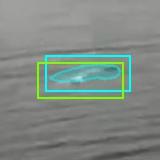
\includegraphics[width=2.45cm]{images/cog/birds1/00003.jpg}}          \hspace{-0.6em}        
    \subfig{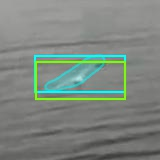
\includegraphics[width=2.45cm]{images/cog/birds1/00005.jpg}}          \hspace{-0.6em}        
    \subfig{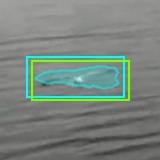
\includegraphics[width=2.45cm]{images/cog/birds1/00007.jpg}}          \hspace{-0.6em}        
    \subfig{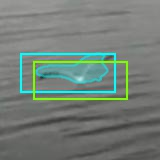
\includegraphics[width=2.45cm]{images/cog/birds1/00013.jpg}}          \hspace{-0.6em}        
    \subfig{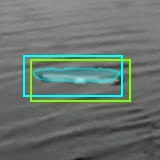
\includegraphics[width=2.45cm]{images/cog/birds1/00057.jpg}}\\[0.2ex]
    \subfig{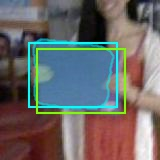
\includegraphics[width=2.45cm]{images/cog/book/00002.jpg}}                     \hspace{-0.6em}
    \subfig{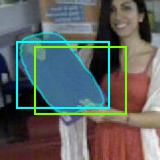
\includegraphics[width=2.45cm]{images/cog/book/00005.jpg}}                     \hspace{-0.6em}
    \subfig{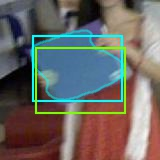
\includegraphics[width=2.45cm]{images/cog/book/00011.jpg}}                     \hspace{-0.6em}
    \subfig{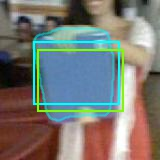
\includegraphics[width=2.45cm]{images/cog/book/00013.jpg}}                     \hspace{-0.6em}    \subfig{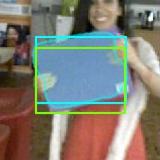
\includegraphics[width=2.45cm]{images/cog/book/00016.jpg}}\\[0.2ex]
    \subfig{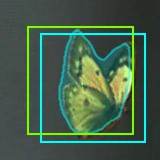
\includegraphics[width=2.45cm]{images/cog/butterfly/00015.jpg}}                   \hspace{-0.6em}
    \subfig{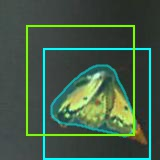
\includegraphics[width=2.45cm]{images/cog/butterfly/00019.jpg}}                   \hspace{-0.6em}
    \subfig{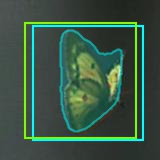
\includegraphics[width=2.45cm]{images/cog/butterfly/00025.jpg}}                   \hspace{-0.6em}
    \subfig{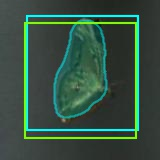
\includegraphics[width=2.45cm]{images/cog/butterfly/00027.jpg}}                   \hspace{-0.6em}
    \subfig{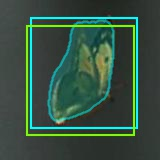
\includegraphics[width=2.45cm]{images/cog/butterfly/00031.jpg}}
    \caption{The tracking result before (green) and after (blue) the instance guided self-correction component.}
    \label{fig:IGSC}
\end{figure}

\subsection{Overview}
\iffalse
For the frame $t$, the tracker uses the observation $o = \{I_t, S_{t-1}\}$, where $I$ is the image of a frame, and $S = \{p, s, h, w\}$ is the state of the tracker. $p$ and $s$ represent the object position and scale in a certain frame; $h$ is the tracking filter and $w$ is the channel reliability. $s_t = T(I_t, S_{t-1})$, where $T$ is the tracker.
\fi
The tracking process (Alg. 1) consists of two phases: localization and model update. 
At the localization phase,  the object position $p_t$ is the position of the maximum in correlation between $h_{t-1}$ and image patch features $f$ extracted on position $p_{t-1}$ and weighted by the channel reliability scores $w$ (Eq. \ref{eq:dcf}).
The segmentation mask $m$ is estimated using the proposed InstMask network (Sect. \ref{sec:InstMask}).
The geometric center of the segmentation mask is used to correct the prediction bias of the correlation filter (Sect. \ref{sec:cog}).
Then the new scale $s_t$ is estimated by a single scale-space correlation filter as in \cite{Danelljan2014AccurateSE}.
The channel detection reliability $\tilde{w}^{(det)}$ is estimated as follows \cite{Lukezic2017DiscriminativeCF}:
\begin{equation} \label{eq:det}
\tilde w_d^{(det)} = max(1 - \rho_d^{max2} / \rho_d^{max1}, 0.5),
\end{equation}
which reflects how uniquely each channel votes for a single target location and used to calculate $w$ later. $\rho_d^{max2}$ and $\rho_d^{max1}$ are the second and first highest non-adjacent peaks in the channel response map, respectively.

At the model update phase, the new filter $\tilde{h}$ is estimated using mask $m$. We use the iterative approach proposed in \cite{Lukezic2017DiscriminativeCF} for efficiently solving the filter. Let $\hat{l}$ be the complex Lagrange multiplier, $\mu > 0$, $h_m=m \odot h$, $\hat{h}^0 = h_{t-1}$ and $\hat{l}^0 = 0$. In each iteration, the following sub-problems are solved sequentially:
\begin{equation} \label{eq:h1}
\hat{h}_c^{i+1} = \frac{\hat{f} \odot \bar{\hat{g}} +(\mu^i \hat{h}_m^i - \hat{l}^i)}{\bar{\hat{f}} \odot \hat f + \mu^i}
\end{equation}
\begin{equation}
h^{i+1} = \frac{m \odot \mathcal{F}^{-1}[\hat{l}^i + \mu^i\hat{h}_c^{i+1}]}{\frac{\lambda}{2D} + \mu^i}
\end{equation}
\begin{equation} \label{eq:h3}
\hat{l}^{i+1} = \hat{l}^i + \mu(\hat{h}_c^{i+1} - \hat{h}^{i+1})
\end{equation}
Then the channel reliability \cite{Lukezic2017DiscriminativeCF} is calculated as follows: 
\begin{equation} \label{eq:c}
\tilde w_d = \tilde w_d^{(lrn)} \cdot \tilde w_d^{(det)},
\end{equation}
where $\tilde{w}^{(lrn)}$ is the learning channel reliability representing the maximum response value of a learned channel filter:
\begin{equation} \label{eq:lrn}
\tilde{w}_d^{lrn} = max(f_d * h_d).
\end{equation}
Finally, the filter and channel reliability are updated online:
\begin{equation} \label{eq:update1}
h_t = (1 - \eta)h_{t-1} + \eta \tilde{h}
\end{equation}
\begin{equation} \label{eq:update2}
w_t = (1-\eta)w_{t-1} + \eta \tilde{w},
\end{equation}
where $\eta$ is the learning rate used to control the speed of model update.

\begin{figure}
    \centering
    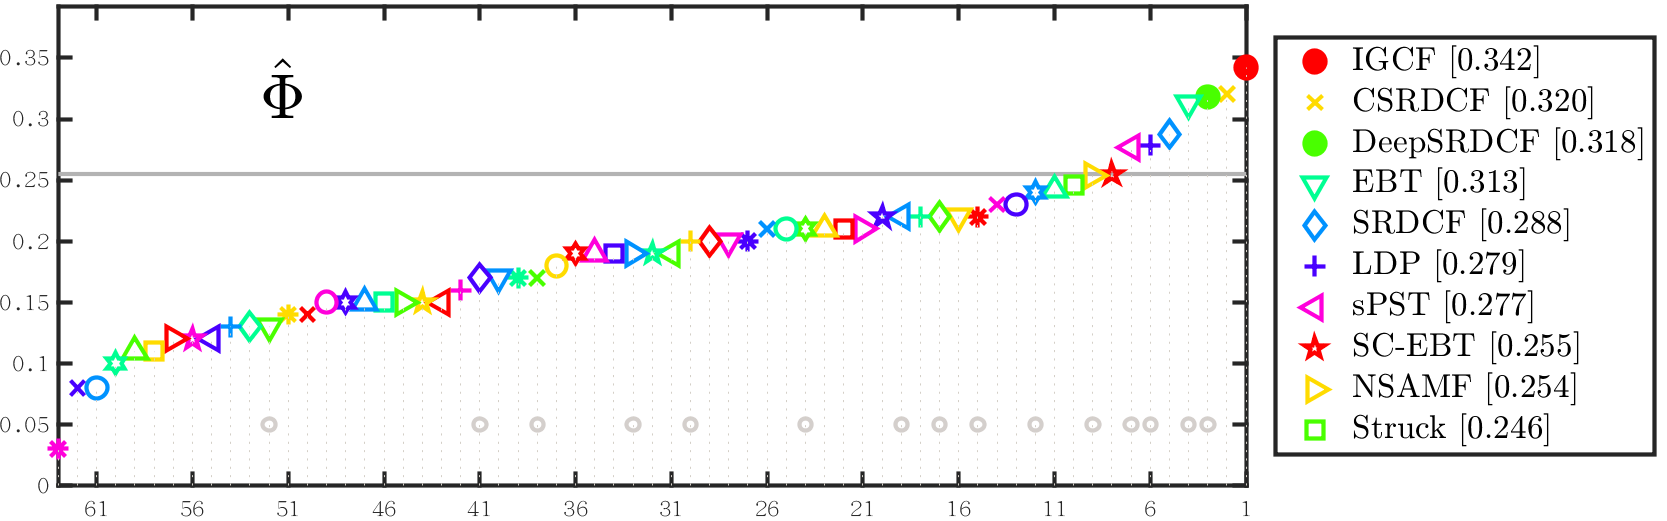
\includegraphics[width=8.8cm]{images/vot/eao_rank_vot2015.png}
    \caption{Expected average overlap (EAO) plot on VOT2015 \cite{Kristan2015TheVO}.}
    \label{fig:vot15}
\end{figure}

\begin{figure}
    \centering
    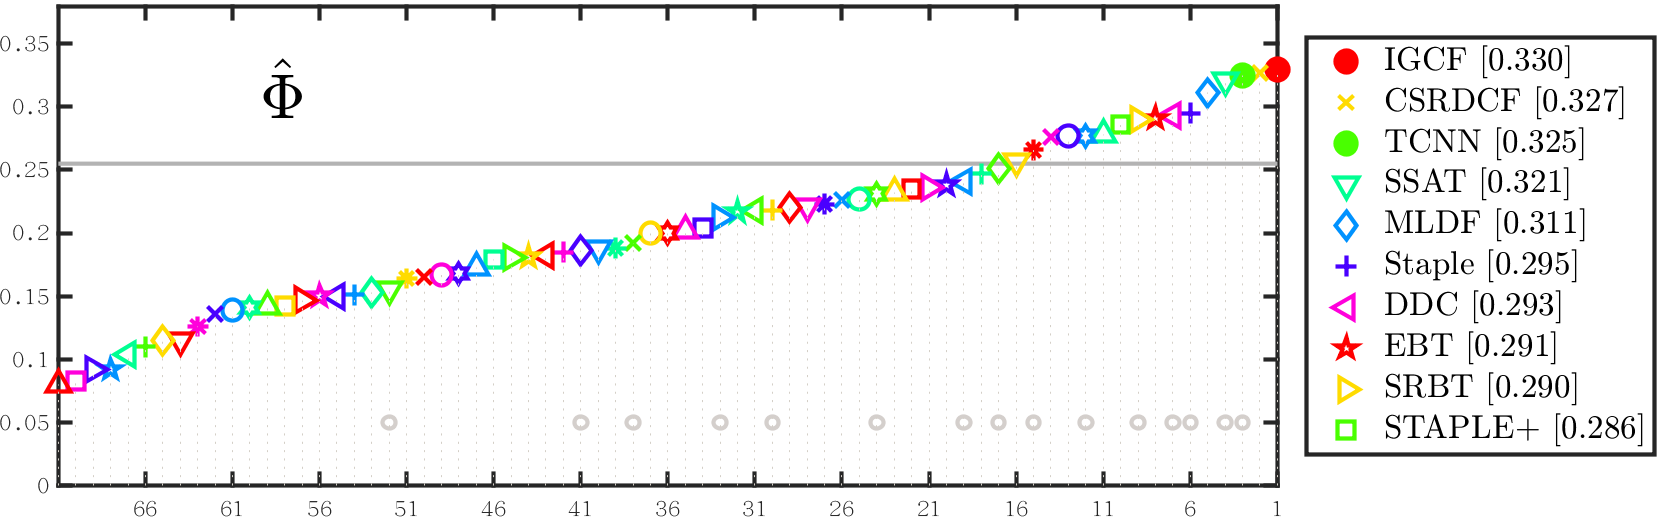
\includegraphics[width=8.8cm]{images/vot/eao_rank_vot2016.png}
    \caption{Expected average overlap (EAO) plot on VOT2016 \cite{Kristan2016TheVO}.}
    \label{fig:vot16}
\end{figure}

\section{Experiments}
We provide a comprehensive evaluation of the proposed tracker IGCF on 3 challenging object tracking datasets: VOT2015 \cite{Kristan2015TheVO}, VOT2016 \cite{Kristan2016TheVO} and GOT-10K \cite{Huang2018GOT10kAL}. Note that there is no overlap between the videos used for training the InstMask component and the evaluation datasets. Besides, a qualitative experiment is carried out on the video object segmentation dataset DAVIS \cite{Perazzi2016}.
\subsection{Evaluation on VOT2015}

\begin{figure}
    \centering
    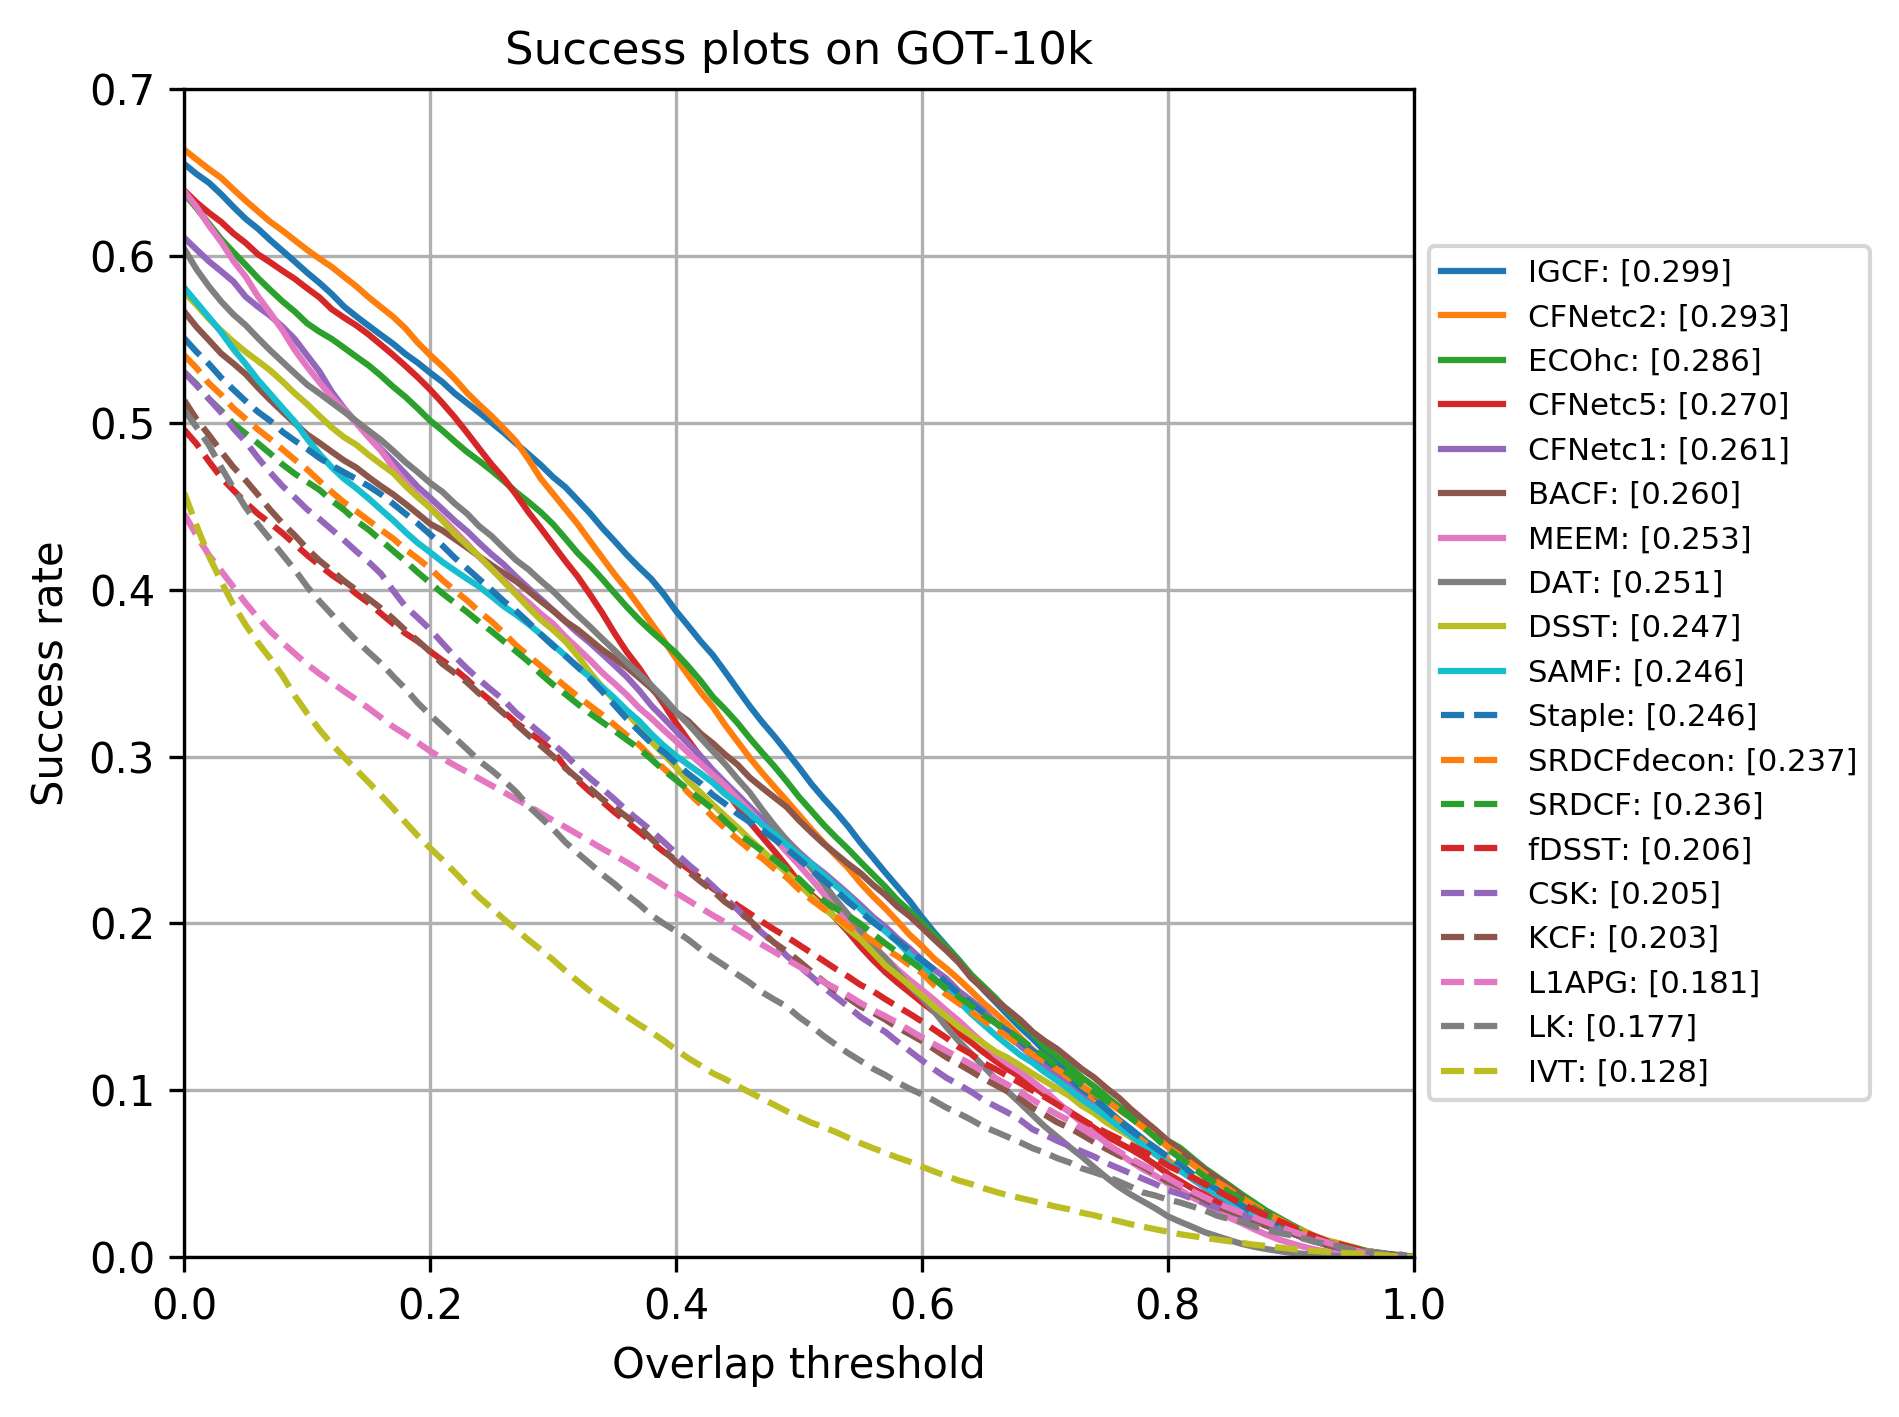
\includegraphics[width=8.8cm]{images/got10k/success_plot.png}
    \caption{Overall performance on GOT-10k \cite{Huang2018GOT10kAL}, ranked by their average overlap (AO) scores.}
    \label{fig:got10k}
\end{figure}

VOT2015 \cite{Kristan2015TheVO} tracking dataset contains 60 challenging videos. and is constructed from over 300 sequences by an advanced sequence selection methodology that favors objects difficult to track and maximizes a visual attribute diversity cost function. In VOT2015, three metrics are used to evaluate the performance of  tracker: (1) accuracy, (2) robustness and (3) EAO (expected average overlap). The accuracy measures how well the bounding box predicted by the tracker overlaps with the ground truth bounding box. The robustness measures how many times the tracker loses the target (fails) during tracking. EAO combines accuracy and robustness to evaluate the overall performance of the tracker. We compare our algorithm with the following trackers: CSRDCF \cite{Lukezic2017DiscriminativeCF}, DeepSRDCF \cite{Danelljan2015ConvolutionalFF}, EBT \cite{Zhu2016BeyondLS}, SRDCF \cite{Danelljan2015LearningSR}, LDP \cite{Kristan2015TheVO}, sPST \cite{Hua2015OnlineOT}, SC-EBT \cite{Hua2015OnlineOT}, NSAMF \cite{Hua2015OnlineOT} and Struck \cite{Hare2011StruckSO}. The EAO scores of the evaluated trackers is shown in Fig. \ref{fig:vot15}. Compared to other listed approaches, our approach achieves a superior EAO of 0.342. Specifically, our approach significantly outperforms the second best tracker CSRDCF with a relative gain of 6.9\% in terms of EAO. This highlights the importance of the proposed InstMask and IGSC modules.

\subsection{Evaluation on VOT2016}
VOT2016 \cite{Kristan2016TheVO} dataset contains 60 sequences from VOT2015 with improved annotations. We compare our algorithm with the following trackers: CSRDCF \cite{Lukezic2017DiscriminativeCF}, TCNN \cite{Kristan2016TheVO}, SSAT \cite{Nam2016LearningMC}, MLDF \cite{Wang2015VisualTW}, Staple \cite{Bertinetto2016StapleC}, DDC \cite{Kristan2016TheVO}, EBT \cite{Zhu2016BeyondLS}, SRBT \cite{Kristan2016TheVO} and STAPLEp \cite{Bertinetto2016StapleC}. Fig. \ref{fig:vot16} shows the EAO performance on the VOT2016. Among the compared methods, our approach achieves the best results with an EAO score of 0.330.

\subsection{Evaluation on GOT-10K}
GOT-10k \cite{Huang2018GOT10kAL} is a large high-diversity database for generic object tracking. We evaluate our tracker on the GOT-10k testing subset which embodies 84 object classes and 32 motion patterns with 180 video segments. The evaluation metric of GOT-10k is average overlap (AO), which  denotes the average of overlaps between all groundtruth and estimated bounding bounding boxes. We compare our algorithm, denoted as IGCF, with the following trackers: CFNetc2 \cite{Valmadre2017EndtoEndRL}, ECOhc \cite{Danelljan2017ECOEC}, CFNetc5 \cite{Valmadre2017EndtoEndRL}, CFNetc1 \cite{Valmadre2017EndtoEndRL}, BACF \cite{Galoogahi2017LearningBC}, MEEM \cite{Zhang2014MEEMRT}, DAT \cite{Possegger2015InDO}, DSST \cite{Danelljan2014AccurateSE}, SAMF \cite{Li2014ASA}, Staple \cite{Bertinetto2016StapleC}, SRDCFdecon \cite{Danelljan2016AdaptiveDO}, SRDCF \cite{Danelljan2015LearningSR}, fDSST \cite{Danelljan2017DiscriminativeSS}, CSK \cite{Henriques2012ExploitingTC}, KCF \cite{Henriques2015HighSpeedTW}, L1APG \cite{Bao2012RealTR}, LK \cite{Shi1994GoodFT} and IVT \cite{Ross2007IncrementalLF}. The success plot of the evaluated trackers is shown in Fig. \ref{fig:got10k}.  The AO score of our method is 0.299, which outperforms all other listed competitive tracking algorithms. 

\begin{figure} 
    \subfig{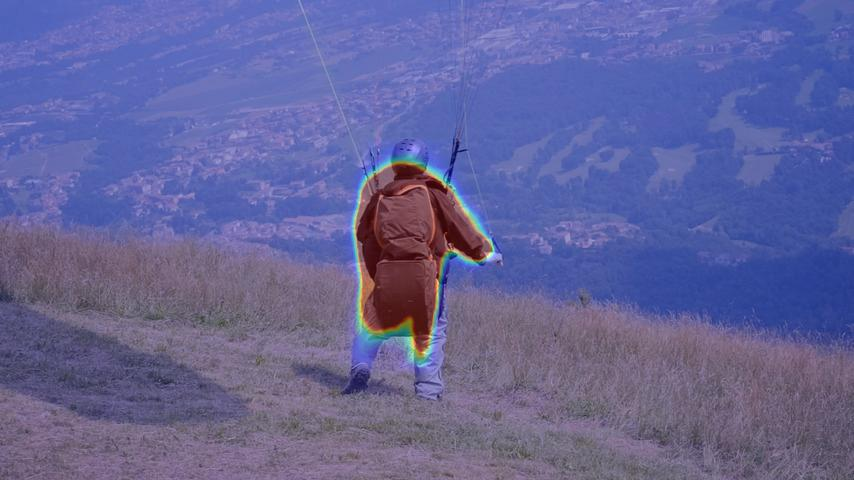
\includegraphics[width=2.43cm]{images/davis16val/paragliding-launch/00001.jpg}}          \hspace{-0.6em}        
    \subfig{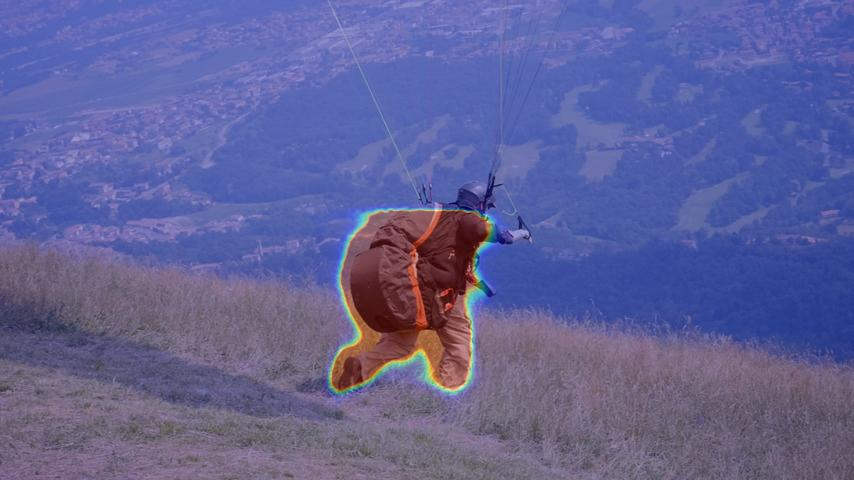
\includegraphics[width=2.43cm]{images/davis16val/paragliding-launch/00021.jpg}}          \hspace{-0.6em}        
    \subfig{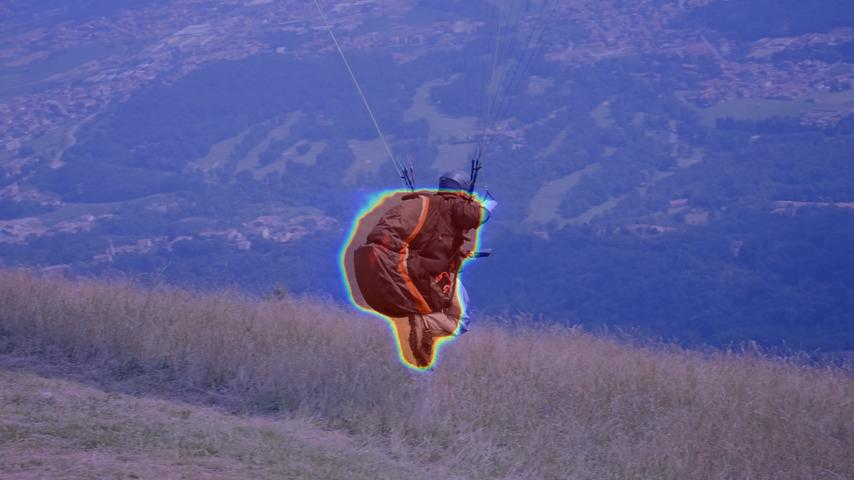
\includegraphics[width=2.43cm]{images/davis16val/paragliding-launch/00032.jpg}}          \hspace{-0.6em}        
    \subfig{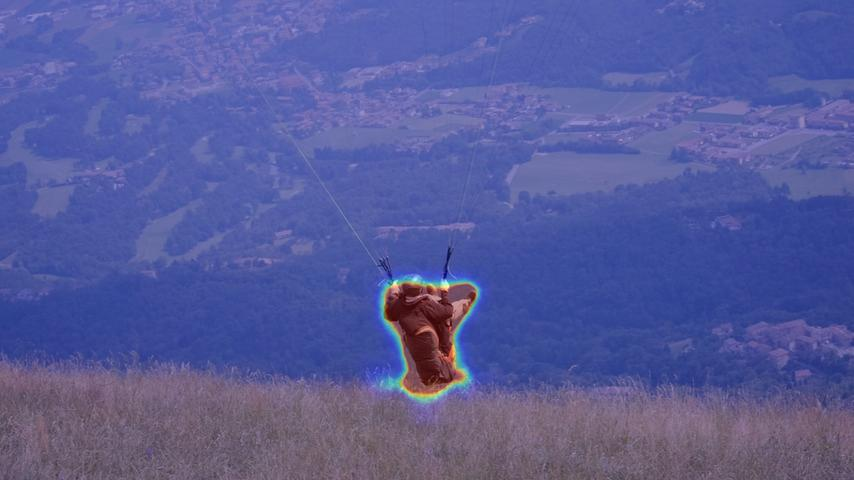
\includegraphics[width=2.43cm]{images/davis16val/paragliding-launch/00069.jpg}}          \hspace{-0.6em}        
    \subfig{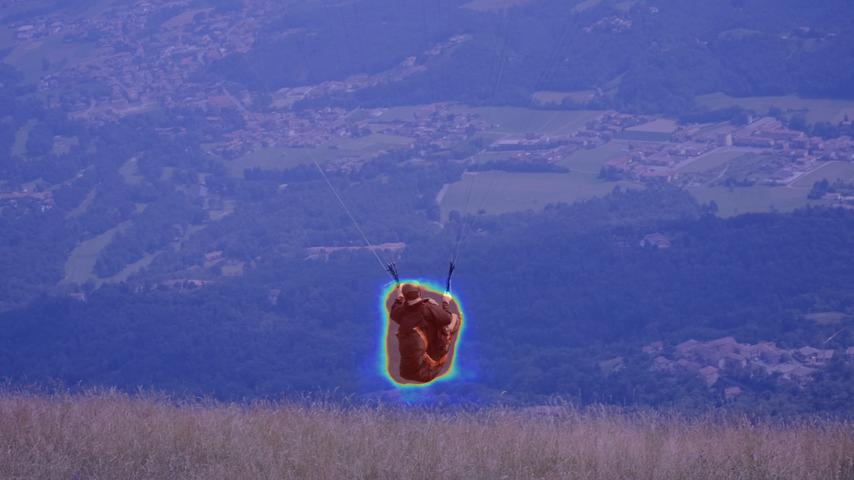
\includegraphics[width=2.43cm]{images/davis16val/paragliding-launch/00079.jpg}}\\[0.2ex]
    \subfig{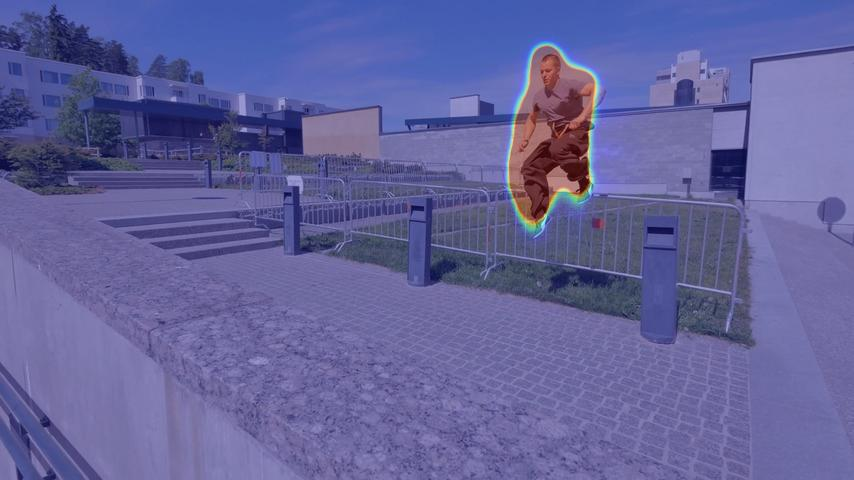
\includegraphics[width=2.43cm]{images/davis16val/parkour/00001.jpg}}                     \hspace{-0.6em}
    \subfig{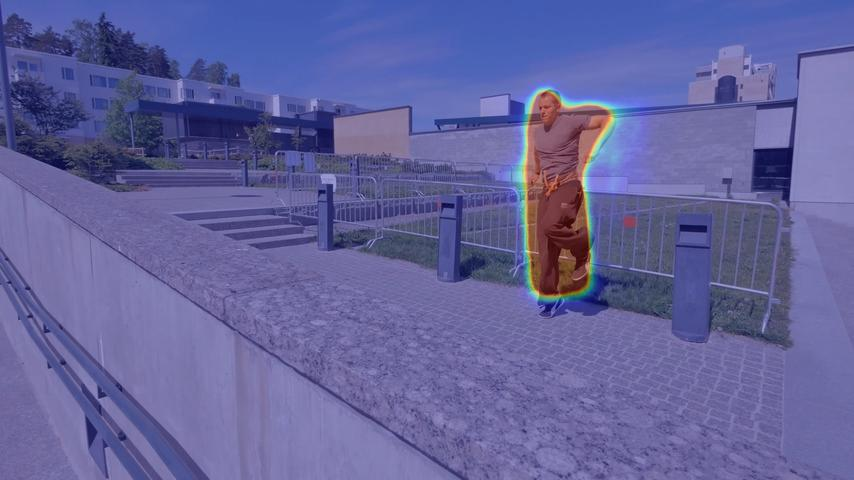
\includegraphics[width=2.43cm]{images/davis16val/parkour/00006.jpg}}                     \hspace{-0.6em}
    \subfig{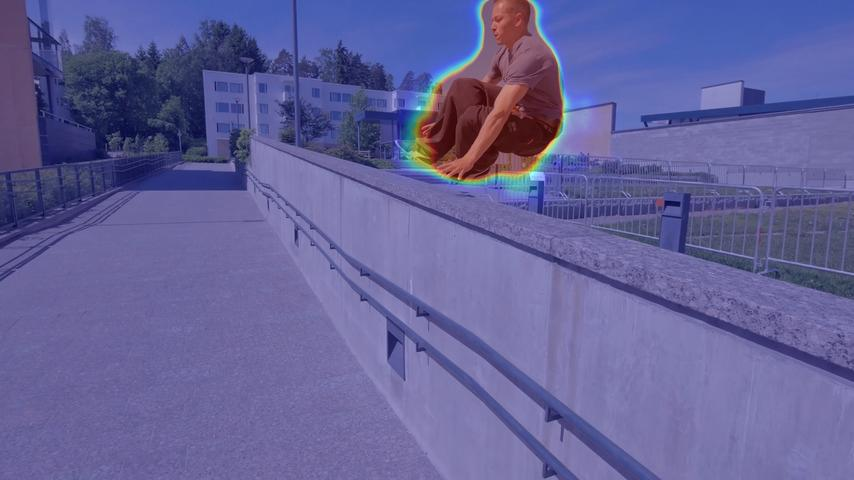
\includegraphics[width=2.43cm]{images/davis16val/parkour/00026.jpg}}                     \hspace{-0.6em}
    \subfig{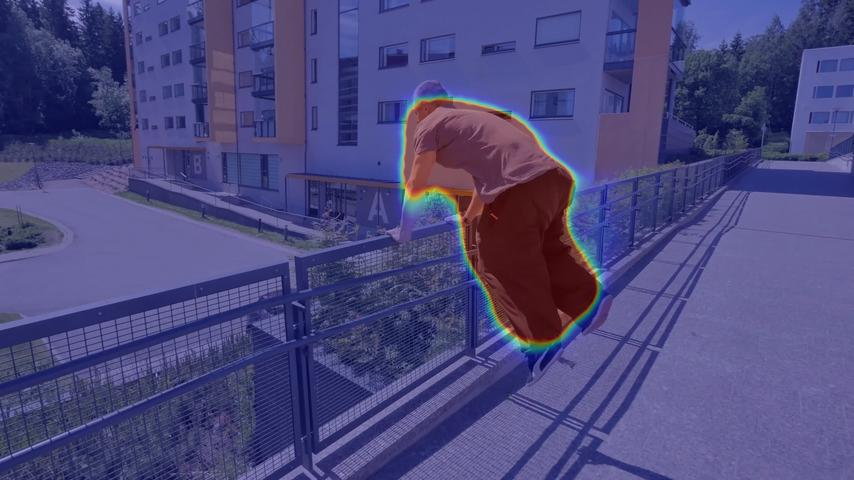
\includegraphics[width=2.43cm]{images/davis16val/parkour/00063.jpg}}                     \hspace{-0.6em}
    \subfig{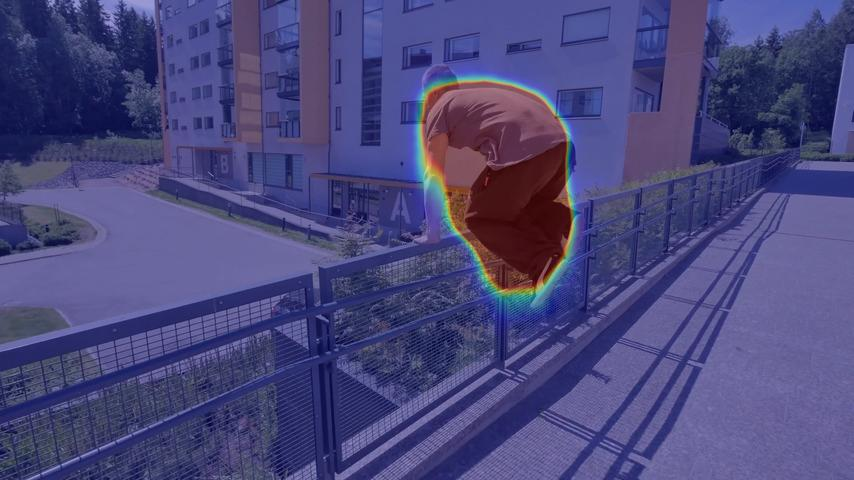
\includegraphics[width=2.43cm]{images/davis16val/parkour/00065.jpg}}\\[0.2ex]
    \subfig{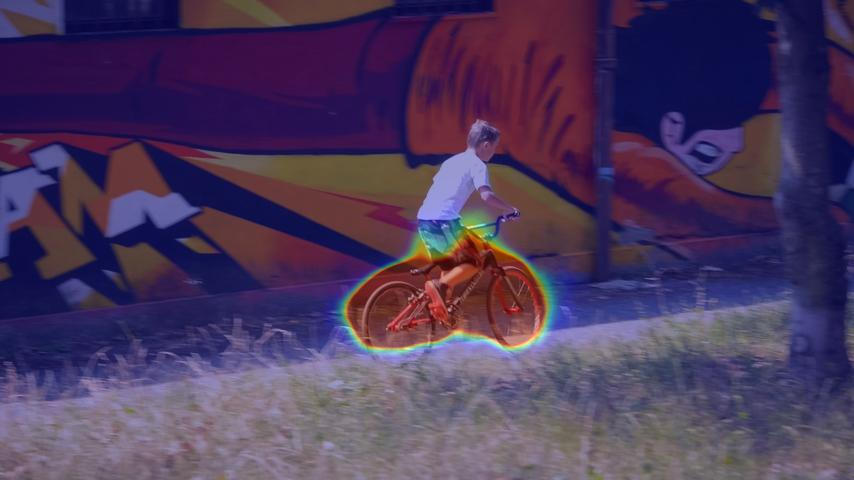
\includegraphics[width=2.43cm]{images/davis16val/bmx-trees/00001.jpg}}                   \hspace{-0.6em}
    \subfig{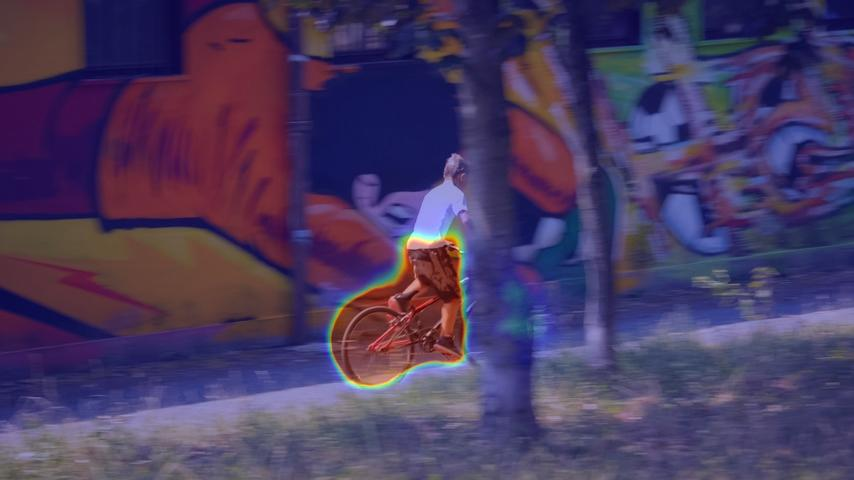
\includegraphics[width=2.43cm]{images/davis16val/bmx-trees/00014.jpg}}                   \hspace{-0.6em}
    \subfig{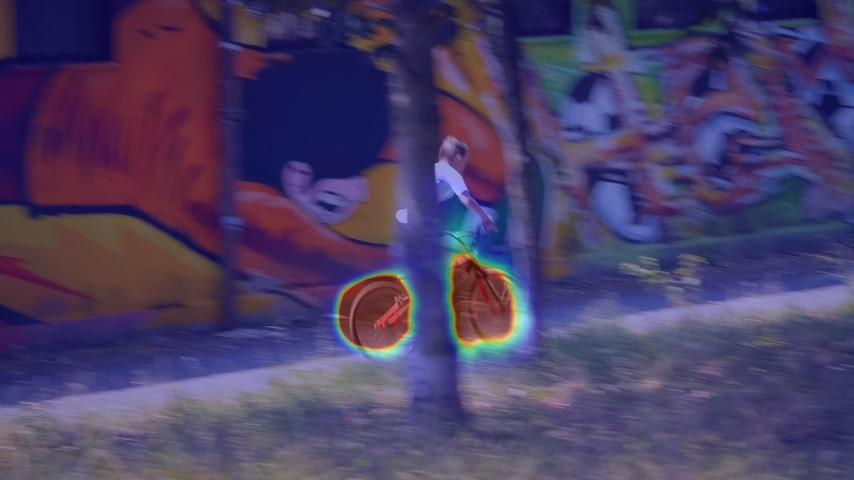
\includegraphics[width=2.43cm]{images/davis16val/bmx-trees/00017.jpg}}                   \hspace{-0.6em}
    \subfig{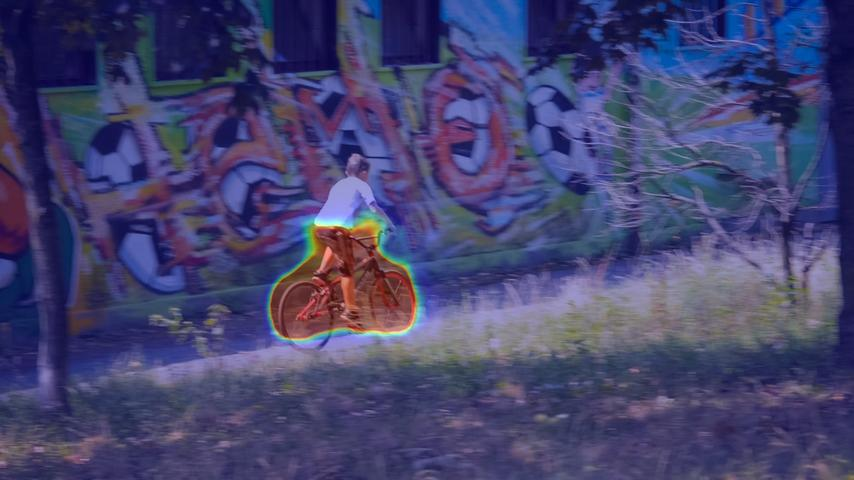
\includegraphics[width=2.43cm]{images/davis16val/bmx-trees/00036.jpg}}                   \hspace{-0.6em}
    \subfig{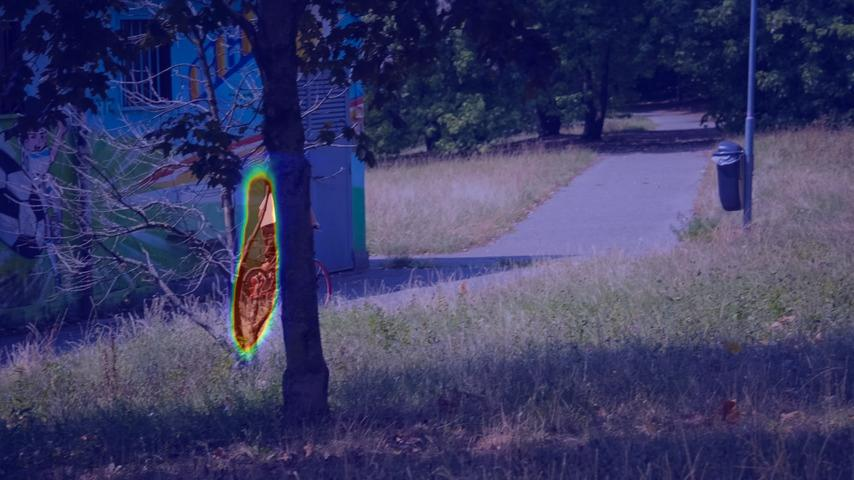
\includegraphics[width=2.43cm]{images/davis16val/bmx-trees/00067.jpg}}
    \caption{Qualitative results of our method in DAVIS2016 VAL dataset.}
    \label{fig:davis}
\end{figure}


\subsection{Evaluation on DAVIS2016}
Equipped with the InstMask module, the proposed not only performs the object tracking task well, but also can be used for the task of video object segmentation. DAVIS \cite{Perazzi2016} is a video object segmentation dataset, which consists of fifty high quality video sequences, spanning multiple occurrences of common video  object segmentation challenges such as occlusions, motion blur and appearance changes. We performed qualitative experiments on the validation set of DAVIS2016. The visualization results are shown in Fig. \ref{fig:davis}. The experimental results show that the proposed IGCF can accurately segment the contour of the object, which explains to some extent the reason why IGCF can achieve performance improvement in the object tracking task.

\section{Conclusion}
In this paper, we propose a novel object tracking model which combines the advantages of deep neural networks and DCF trackers to improve the performance of object tracking.
The InstMask are used to explicitly constraint the learning process of correlation filters. Based on the instance-level segmentation, we further propose a self-correction mechanism to mitigate the drift problem of CF trackers.
The segmentation result from CNN can effectively correct the unstable drift of DCF.
Experiment results exhibit the superior robustness and efficiency of the proposed method by comparing with state-of-the-art trackers.

\section*{References}

\bibliography{mybibfile}

\end{document}